\problemname{Spock}

%\illustration{0.35}{nimoy}{Photo by Gage Skidmore via \href{http://commons.wikimedia.org/wiki/File:Leonard_Nimoy_by_Gage_Skidmore_3.jpg}{Wikimedia Commons}}
Leo is participating in a friendly game of
\emph{rock-paper-scissors-lizard-Spock} against his computer.  The
game proceeds in rounds.  In each round, Leo and his computer both
choose, simultaneously, between five options: rock, paper, scissors,
lizard, and Spock.  Each of these five options wins over two of the
other options, as illustrated by Figure~\ref{fig:rpsls}.  For example,
rock wins over lizard and scissors, but loses against paper and Spock.
If both players choose the same option, the round is a draw.
In the end, each of the two players gets a score which is the number
of rounds they won.

\begin{figure}[!h]
  \centering
  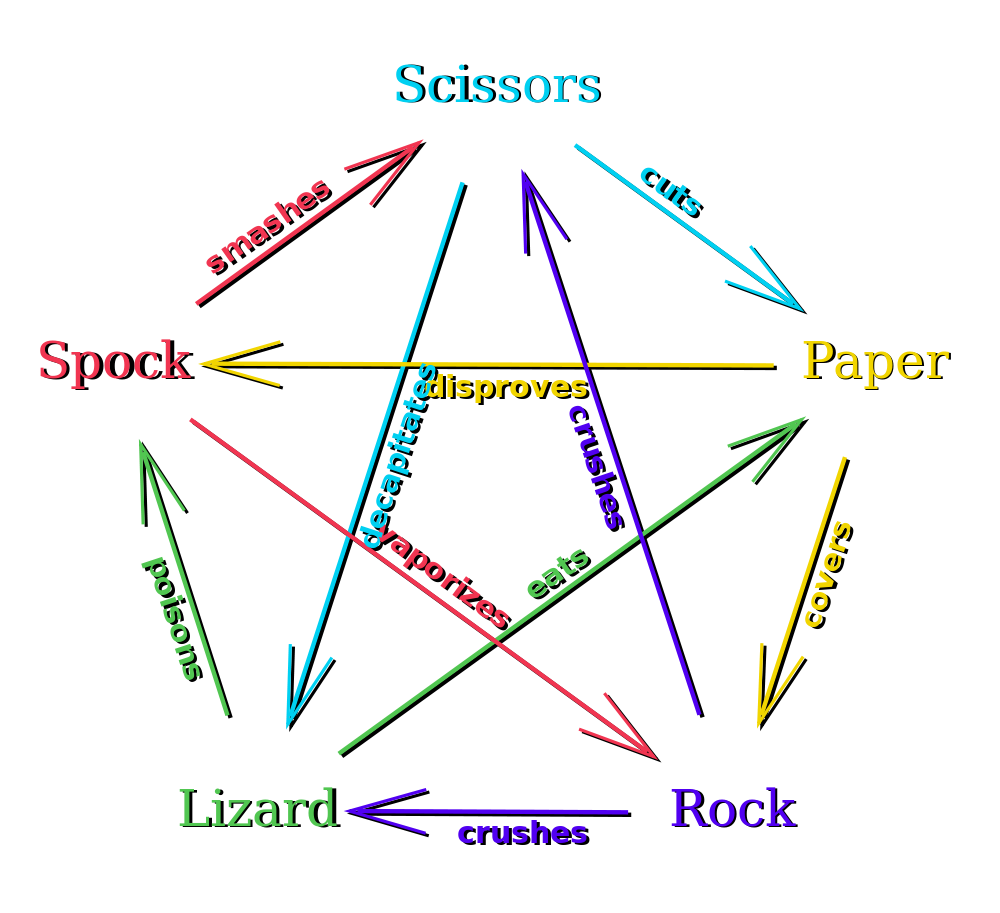
\includegraphics[width=0.4\textwidth]{rpsls}
  \caption{The mechanics of the game.  Illustration by VidTheKid via \href{http://commons.wikimedia.org/wiki/File:Rock_Paper_Scissors_Lizard_Spock_en.svg}{Wikimedia Commons}}
  \label{fig:rpsls}
\end{figure}

Alas, Leo's computer is not the sharpest tool in the shed, and simply
follows a strategy where in each round it selects one of the five
options uniformly at random.  This makes the game quite boring,
because regardless of Leo's strategy, each player is expected to win
$40\%$ of the rounds (and $20\%$ of the rounds are expected to be
draws). 

Did we mention that Leo's computer is a bit lacking in mental
capacities already?  Well, it gets worse: in order to pick random
options, Leo's computer uses a very simple linear congruential
generator (LCG).  The LCG has three parameters: a \emph{known} prime number $p =
127$, and two fixed but \emph{unknown} integers $0 \le a < p$ and $0
\le b < p$.  Additionally, it has a state, an integer $0 \le x < p$.
To generate a random option, Leo's computer first updates the state
according to the rule
\[
x \leftarrow (a \cdot x + b) \bmod p,
\]
and then chooses one of the five options based on the value of $x
\bmod 5$, according to the following table:

\begin{center}
\begin{tabular}{|c|c|c|c|c|c|}
\hline
$x \bmod 5$: & $0$ & $1$ & $2$ & $3$ & $4$ \\
\hline
Option chosen: & rock & paper & scissors & lizard & Spock \\
\hline
\end{tabular}
\end{center}

Logically, knowing how Leo's computer chooses its random numbers
should give Leo an advantage in the game.  But unfortunately Leo died,
so it is now up to you to finish this.  Write a program which, when
playing against Leo's computer for several rounds, wins at least
$80\%$ of them.


\section*{Interaction}

This problem is interactive, proceeding in the rounds of the game.
Before the game starts, there will be one line of input containing an
integer $100 \le r \le 1000$, the number of rounds to play.

Then, for each round, your program should write one line containing
one of the five strings ``\texttt{rock}'', ``\texttt{paper}'',
``\texttt{scissors}'', ``\texttt{lizard}'', or ``\texttt{Spock}'',
indicating the option Leo should choose for the next round.  After
writing this line you need to make sure to flush standard output.
Then, one line of input will be available, containing the name of the
option chosen by Leo's computer in the round, and the game proceeds to
the next round.

A Java jar file \href{http://challenge.csc.kth.se/2015/SpockDebugger.jar}{SpockDebugger.jar} is provided to aid in testing your solution. Running
\texttt{java -jar SpockDebugger.jar} in a terminal gives information about usage.

\section*{Sample Interaction}

Suppose that Leo's computer uses the parameters $a = 17$, $b = 23$,
and is initially in state $x = 42$.  Then in the first round, the
state is updated to $(17 \cdot 42 + 23) \bmod 127 = 102$, and since
$102 \bmod 5 = 2$, the first move made by the computer is
\texttt{scissors}.  In the next round, the state is updated to $(17
\cdot 102 + 23) \bmod 127 = 106$, resulting in the move
\texttt{paper}.  The first $10$ rounds of the game are shown below.
In this example, Leo has opted to simply make the move \texttt{Spock}
in every single round, which seems to have been a surprisingly good
choice -- of these $10$ rounds Leo actually wins $7$ (all but the
second, sixth, and seventh) -- but Leo still is not winning $80\%$ of
the rounds.  In general, this strategy will be too naive to defeat
the computer.

The extra newlines in this example are for clarity only, to
demonstrate the order of events.  You should print exactly one newline
character after each move, and the input contains no blank lines
either.


\ifplastex % I have no clue why but for some reason this works but just doing the include does not... /Per
\displaysample{spock/problem_statement/sample}
\else
\displaysample{spock/problem_statement/sample}
\fi
